\section{2020 年 9 月 26 日答疑记录}

\subsection{简单的分式不等式的解法}

关于 $x$ 的形如 $\dfrac{Ax+B}{Cx+D}>(\geqslant)\,0$ 的分式不等式, 可以利用分子和分母的正负号关系转化为二次不等式来解. 具体地,
\begin{align}\label{eq-201009-1907}
  \frac{Ax+B}{Cx+D}>0 & \Leftrightarrow (Ax+B)(Cx+D)>0,\\
  \label{eq-201009-1917}
  \frac{Ax+B}{Cx+D}\geqslant 0 & \Leftrightarrow \left\{\!\!
    \begin{array}{l}
      (Ax+B)(Cx+D)\geqslant 0,\\
      Cx+D\neq 0.
    \end{array}\right.
\end{align}
\eqref{eq-201009-1907} 式中右边不用限制分母非零, 因为乘积非零隐含两个因子均非零; 而 \eqref{eq-201009-1917} 式中右边必须限制分母非零, 因为乘积为零隐含两个因子均可能为零. 

\begin{example}
  解下列不等式:
  \begin{twocolpro}
    (1) $\dfrac{x-2}{x-5}>0$; & (2) $\dfrac{x-2}{x-5}\geqslant 0$.
  \end{twocolpro}
\end{example}
\begin{solution}
  (1) 原不等式等价于 $(x-2)(x-5)>0$, 所以 $x\in (-\infty,2)\cup (5,+\infty)$.
  
  (2) 原不等式等价于
  \[\left\{\!\!\begin{array}{l}
        (x-2)(x-5)\geqslant 0,\\
        x-5\neq 0,
      \end{array}\right. \text{解得}\ 
      x\in (-\infty,2]\cup (5,+\infty).\]
\end{solution}

解二次不等式时, 需要考虑对应抛物线的图象, 尤其应注意开口方向. 也可以先将不等式各因子化为最高次项系数为正的形式, 然后再根据抛物线的图象写出相应的解集.

\begin{example}
  解下列不等式:
  \begin{twocolpro}
    (1) $\dfrac{2-x}{x-5}>0$; & (2) $\dfrac{2-x}{x-5}\geqslant 0$.
  \end{twocolpro}
\end{example}
\begin{solution}
  (1) 原不等式等价于 $(2-x)(x-5)>0$ 即 $(x-2)(x-5)<0$ , 所以 $x\in (2,5)$.
  
  (2) 原不等式等价于
  \[\left\{\!\!\begin{array}{l}
        (2-x)(x-5)\geqslant 0,\\
        x-5\neq 0,
      \end{array}\right. \text{解得}\ 
      x\in [2,5).\]
\end{solution}

关于 $x$ 的形如 $\dfrac{Ax+B}{Cx+D}>(\geqslant)\,E$ 的分式不等式, 也可以改写为
\[\frac{Ax+B}{Cx+D}-E>(\geqslant)\,0\quad \text{即}\quad
  \frac{Ax+B-E(Cx+D)}{Cx+D}>(\geqslant)\,0,\]
从而化为前面形式的不等式来求解.

\begin{example}
  解下列不等式:
  \begin{twocolpro}
    (1) $\dfrac{2x-3}{x-5}>1$; & (2) $\dfrac{2-x}{x-5}\geqslant 2$.
  \end{twocolpro}
\end{example}
\begin{solution}
  (1) 原不等式化为
  \[\frac{2x-3}{x-5}-1>0\quad \text{即}\quad \frac{x+2}{x-5}>0,\] 
  所以等价于 $(x+2)(x-5)>0$, 解得 $x\in (-\infty,-2)\cup (5,+\infty)$.
  
  (2) 原不等式化为
  \[\frac{2-x}{x-5}-2\geqslant 0\quad \text{即}\quad \frac{12-3x}{x-5}\geqslant 0,\] 
  所以等价于
  \[\left\{\!\!\begin{array}{l}
        (12-3x)(x-5)\geqslant 0,\\
        x-5\neq 0,
      \end{array}\right. \text{解得}\ 
      x\in [4,5).\]
\end{solution}

\subsection{绝对值的几何意义}

实数 $a$ 的绝对值定义为
\[|a|=\begin{cases}
  a, & a>0,\\
  0, & a=0,\\
  -a, & a<0
  \end{cases}= \begin{cases}
    a, & a\geqslant 0,\\
    -a, & a<0,
    \end{cases}\]
其几何意义为数轴上坐标为 $a$ 的点到原点的距离. 进而可以知道, 数轴上两点 $x_1$, $x_2$ 之间的距离为 $|x_1-x_2|$, 如下图所示.

\begin{center}
  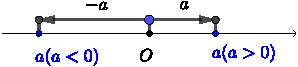
\includegraphics[scale=1]{2020-1009-2110-crop}\qquad
  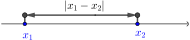
\includegraphics[scale=1]{2020-1009-2120-crop}
\end{center}

例如, $|x-1|$ 表示点~$x$ 到 $1$ 的距离; $|x+2|=|x-(-2)|$ 表示点~$x$ 到 $-2$ 的距离; $|2x-2|= 2|x-1|$ 表示点~$x$ 到 $1$ 的距离的 $2$~倍; $|4+2x|= 2|x-(-2)|$ 表示点~$x$ 到 $-2$ 的距离的 $2$~倍. 注意, 前面运用了绝对值的运算法则: $|ka|= |k|\,|a|$ (为什么?).

再由勾股定理可知, 平面直角坐标系中两点 $A(x_A,y_A)$, $B(x_B,y_B)$ 之间的距离为
\begin{align*}
  AB&= \sqrt{CD^2+EF^2}
     = \sqrt{|x_A-x_B|^2+|y_A-y_B|^2}\\
    &= \sqrt{(x_A-x_B)^2+(y_A-y_B)^2}.
\end{align*}

\begin{center}
  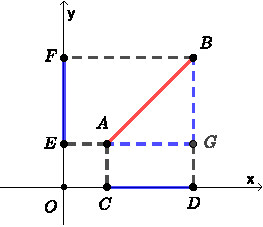
\includegraphics[scale=1]{2020-1009-2130-crop}
\end{center}

函数 $y=|x|$ 的图象可以通过描点画图或图象变换 (即先画 $y=x$ 的图象, 再把 $x$~轴下方的部分关于 $x$~轴对称翻折到 $x$ 轴上方) 得到, 如下图所示:

\begin{center}
  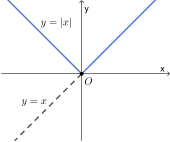
\includegraphics[scale=1]{2020-1011-1000-crop}
\end{center}

一般的, $y= |f(x)|$ 的图象可以由 $y=f(x)$ 的图象经过变换得到, 如下图所示:

\begin{center}
  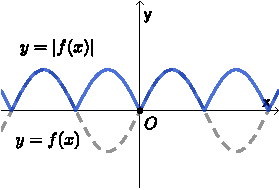
\includegraphics[scale=1]{2020-1011-1010-crop}
\end{center}

简单的带绝对值的不等式, 可以根据绝对值的几何意义直接求解. 如不等式 $|x|<3$, 由 $|x|$ 表示点~$x$ 到原点的距离可知,  $x\in (-3,3)$; 而由不等式 $|x|\geqslant 3$, 可解得 $x\in(-\infty,-3]\cup[3,+\infty)$.

\begin{example}
  解下列不等式:
  \begin{threecolpro}
    (1) $|x-1|\leqslant 2$; & (2) $|2x+1|> 3$; & (3) $|1-2x|\geqslant 5$.
  \end{threecolpro}
\end{example}
\begin{solution}
  (1) 由题可将 $x-1$ 视为整体, 则 $-2\leqslant x-1\leqslant 2$, 即 $-1\leqslant x\leqslant 3$, 所以 $x\in [-1,3]$.
  
  (2) 由题, $2x+1<-3$ 或 $2x+1>3$, 即 $x<-2$ 或 $x>1$, 所以 $x\in(-\infty,-2)\cup (1,+\infty)$.
  
  (3) 由题, $1-2x\leqslant -5$ 或 $1-2x\geqslant 5$, 即 $x\geqslant 3$ 或 $x\leqslant -2$, 所以 $x\in(-\infty,-2]\cup [3,+\infty)$.
\end{solution}

稍微复杂一些的带绝对值的不等式, 有的也可以根据绝对值的几何意义来求解. 只含一个绝对值的不等式, 可以按绝对值的几何意义适当讨论; 含两个绝对值的不等式, 讨论起来麻烦一点, 可以先尝试不等式两边平方.

\begin{example}
  解下列不等式:
  \begin{threecolpro}
    (1) $|x+1|<2x$; & (2) $|x-1|\geqslant 2x$; 
    & (3) $|2x+1|> |x|$.
  \end{threecolpro}
\end{example}
\begin{solution}
  (1) 由题意,
  \[\left\{\!\!\begin{array}{l}
    2x>0,\\
    -2x<x+1<2x,
  \end{array}\right.\text{解得}\ x\in(1,+\infty).\]
  
  (2) 若 $2x\leqslant 0$ 即 $x\leqslant 0$, 则不等式已成立. 
  
  若 $2x> 0$ 即 $x> 0$, 则不等式等价于 
  \[x-1\leqslant -2x\quad \text{或}\quad x-1\geqslant 2x,\]
  解得 $x\leqslant \dfrac13$ 或 $x\leqslant -1$. 结合 $x>0$ 知, 此时 $0<x\leqslant \dfrac13$. 
  
  综上所述, $x\in\biggl(-\infty,\dfrac13\biggr]$.
  
  (3) 不等式两边平方得 
  \[(2x+1)^2>x^2\quad \text{即}\quad (x+1)(3x+1)>0,\]
  解得 $x\in(-\infty,-1)\cup \biggl(\dfrac13,+\infty\biggr)$.
\end{solution}
